
%(BEGIN_QUESTION)
% Copyright 2009, Tony R. Kuphaldt, released under the Creative Commons Attribution License (v 1.0)
% This means you may do almost anything with this work of mine, so long as you give me proper credit

A fish hatchery adds salt to the water in the rearing ponds to enhance fish growth at certain stages in their development.  A P\&ID shows the layout of the control system:

$$\includegraphics[width=15.5cm]{i00924x01.eps}$$


\begin{itemize}
\item{} What type of analyzer technology (e.g. pH, NDIR, gas chromatograph, conductivity, fluorescence, etc.) would be most practical for measuring the salt content of the water?
\vskip 40pt
\item{} Assuming direct action on the part of the transmitter and a signal-to-open water valve, which control action ({\it direct} or {\it reverse}) should the controller be configured for?
\vskip 40pt
\item{} How will the control system respond to an {\it increase} in salt feed rate added to the rearing pond? 
\vskip 40pt
\item{} Suppose the AT fails with a low (4 mA) signal with the controller in automatic mode.  How will this affect the actual salinity of the water over time?
\end{itemize}

\underbar{file i00924}
%(END_QUESTION)





%(BEGIN_ANSWER)

\begin{itemize}
\item{} What type of analyzer should the transmitter (AT) be (e.g. pH, NDIR, gas chromatograph, conductivity, SO$_{2}$ fluorescence, etc.) to properly measure salt content in the water?  {\bf Conductivity}
\vskip 10pt
\item{} Assuming direct action on the part of the transmitter and a signal-to-open water valve, which control action ({\it direct} or {\it reverse}) should the controller be configured for?  {\bf Direct action}
\vskip 10pt
\item{} How will the control system respond to an {\it increase} in salt feed rate added to the rearing pond?  {\bf Increasing fresh water flow to the pond to maintain constant salinity}
\vskip 10pt
\item{} Suppose the AT fails with a low (4 mA) signal with the controller in automatic mode.  How will this affect the actual salinity of the water over time?  {\bf The controller will saturate its output low, stopping all water to the pond.  The result will be excessive salinity and stagnation of the water.}
\end{itemize}

I recommend 2 points each for the first two answers, and 3 points each for the last two answers.

%(END_ANSWER)





%(BEGIN_NOTES)

{\bf This question is intended for exams only and not worksheets!}.

%(END_NOTES)
